\documentclass[czech,bachelor,dept460,male,csharp,cpdeclaration]{diploma}

\usepackage[autostyle=true,czech=quotes]{csquotes} % korektni sazba uvozovek, podpora pro balik biblatex
\usepackage[backend=bibtex, style=iso-numeric, alldates=iso]{biblatex} % bibliografie
\usepackage{dcolumn} % sloupce tabulky s ciselnymi hodnotami
\usepackage{subfig} % makra pro "podobrazky" a "podtabulky"

\usepackage{geometry}
\usepackage{listings}

%\usepackage{mathtools} %- blokuje list obrázků a tabulek

\ThesisAuthor{Jan Jedlička}

\ThesisSupervisor{Ing. Jan Janoušek}

\CzechThesisTitle{Webová služba pro sběr a vizualizaci předpovědí počasí}

\EnglishThesisTitle{Web Service for Collection and Visualization of Weather Forecasts}

\SubmissionYear{2021}

\Acknowledgement{Rád bych na tomto místě poděkoval vedoucímu bakalářské práce panu Ing. Janu Janouškovi, za pravidelné konzultace a poskytnutí mnoha užitečných rad a nápadů pro řešení samotné práce.}

% Zadame cestu a jmeno souboru ci nekolika souboru s digitalizovanou podobou zadani prace.
% Pokud toto makro zapoznamkujeme sazi se stranka s upozornenim.
%\ThesisAssignmentImagePath{Figures/Assignment}

% Zadame soubor s digitalizovanou podobou prohlaseni autora zaverecne prace.
% Pokud toto makro zapoznamkujeme sazi se cisty text prohlaseni.
%\AuthorDeclarationImageFile{Figures/AuthorDeclaration.jpg}


% Zadame soubor s digitalizovanou podobou souhlasu spolupracujici prav. nebo fyz. osoby.
% Pokud toto makro zapoznamkujeme sazi se cisty text souhlasu.
%\CooperatingPersonsDeclarationImageFile{Figures/CoopPersonDeclaration.jpg}

\CzechAbstract{Cílem bakalářské práce bylo vytvořit knihovnu, která bude schopna shromažďovat data o počasí z různých datových zdrojů v různých formátech (text XML, text JSON, bitmap). Agregovaná data jsou následně poskytována pomocí webové služby v jednom formátu (bitmap). Webová služba poskytuje data pro určité území v daném čase. Posledním bodem je vizualizační aplikace, která poskytuje uživateli možnost vykreslení počasí pro určité území v čase a také zobrazuje předpověď pro zadanou trasu.}

\CzechKeywords{XML; JSON; bitmap; počasí}

\EnglishAbstract{The aim of the bachelor thesis was to create a library that will be able to collect weather data from various data sources in various formats (XML text, JSON text, bitmap). The aggregated data is then provided using a web service in one format (bitmap). The web service provides data for a specific territory at a given time. The last point is a visualization application that provides the user with the ability to plot the weather for a certain area over time and also displays the forecast for the specified route.}

\EnglishKeywords{XML; JSON; bitmap; forecast}

\AddAcronym{XML}{Extensible Markup Language}
\AddAcronym{JSON}{JavaScript Object Notation}
\AddAcronym{BMP}{Bitmap}
\AddAcronym{API}{Application Programming Interface}
\AddAcronym{Typ počasí}{Druh meteorologického prvku}
\AddAcronym{Loader}{Knihovna reprezentující jeden z datových zdrojů}

\addbibresource{citace.bib}

% Zacatek dokumentu
\begin{document}
	
	\MakeTitlePages
	
	\chapter{Úvod}
	
	Informace o počasí jsou v dnešní době distribuovány mnoha službami v různých podobách. Nejčastěji narážíme na textové formáty (XML/JSON) kde zprostředkovatelé dodávají kompletní výpis informací pro stát, město nebo konkrétní bod na základě zeměpisných souřadnic. Mimo textový formát narážíme i na snímky z radaru či barevné bitmapy, které poskytují předpověď pro rozsáhlou plochu v konkrétním čase. Předpovědi jsou vytvářeny pro různé časové intervaly na rozdílnou dobu dopředu, můžete tedy například narazit na předpověď obsahující data na 24 hodin dopředu s hodinovými rozestupy nebo na týden s vzájemnými rozestupy šesti hodin. Vzhledem k tomu že ke změnám počasí dochází relativně pomalu tak není potřeba znát data pro každou sekundu či minutu, stačí nám předpověď jednou za pár desítek minut případně i pár hodin.
	
	Cílem této práce je tedy sjednotit různé datové zdroje do jednotného formátu a vytvořit předpověď počasí pro určitou plochu v čase dle průměru těchto dat. Mimo to, že každá služba může mít data ve svém formátu, je potřeba i sjednotit časy a především pozice pro které se data zjišťují.
	
	Dalším úkolem je vytvořit službu která bude schopna tyto agregovaná data poskytovat na základě dotazů uživatele. Uživatel může žádat o poskytnutí dat pro určitou plochu v patřičném čase, čímž obdrží patřičnou bitmapu. Případně může zažádat o předpověď v jednom bodě pro jeden či více časů s různými rozestupy.
	
	Nakonec práce se musí vytvořit aplikace, která nám zobrazí agregovaná data z naší služby a otestuje veškeré potřebné dotazy. Převede hodnoty z bitmap zpět na patřičné číselné údaje, zobrazí různé meteorologické prvky počasí pro zvolené časy a plochu ať už pro jeden bod nebo trasu tvořenou desítkami různých míst.
	
	\chapter{Datové zdroje}
	
	V práci je zapotřebí použít minimálně 3 různé datové zdroje. Jako první se tedy zvolil norský datový zdroj poskytovaný serverem yr.no, který dodává data v podobě XML textu. Druhým zvoleným zdrojem jsou JSON předpovědi od společností OpenWeather a WeatherUnlocked. Poslední zdroj poskytuje data ve formě bitmap reprezentujících přímo snímky z radaru nebo předem zpracované bitmapy hodnot a pro tento účel byl vybrán český projekt Medard a Radar bouřky.
	
	\section{XML}
	
	Prvním zpracovávaným typem je XML. XML je způsob formátování dat v textové podobě, který nám v tomto případě poskytuje data o počasí mnoha meteorologických prvků pro jedno místo ve více časech. Tento formát se postupně nahrazuje modernějším typem JSON, nicméně služby poskytují zpětnou kompatibilitu a možnost získávat data stále v tomto formátu.
	
	\subsection{Yr.no}
	
	Tímto datovým zdrojem je norská meteorologická služba zvaná Yr \cite{yrno}. Poskytují data o počasí pokrývající celý svět, lze si stáhnout data pro určité město pomocí zadání jeho názvu nebo bod založený na zeměpisných souřadnicích. Předpovědi jsou vždy od aktuálního času na 9 dnů dopředu a rozpětí mezi jednotlivými předpověďmi je 1 hodina pro následující 3 dny a 6 hodin pro zbylých 6 dnů. Předpověď vždy začíná od aktuálního času zaokrouhleného na hodiny dolů. Veškeré informace jsou v podobě XML případně JSON dokumentu. V práci se využívá XML formát pro ukázku využití odlišných forem předání dat, i když JSON formát je praktičtější a preferovanější z důvodů jako je snazší deserializace a potřeba stáhnout objemově mnohem méně dat.
	
	Při využívání této služby se používá API, které pro zadaný bod vrací počasí. To znamená že pro určení dat stačí znát pouze zeměpisné souřadnice zvoleného bodu a ty zadat jako parametry {\it lon} a {\it lat}.
	
	Ukázka odkazu který vrací XML text obsahující data o počasí pro Ostravu na následujících 9 dnů.
	\begin{itemize}
		\item \url{https://api.met.no/weatherapi/locationforecast/2.0/classic?lat=49.820923\&lon=18.262524}
	\end{itemize}
	
	\section{JSON}
	
	Druhým zpracovávaným typem předpovědí v textové podobě je JSON, který obsahuje rovněž data o mnoha různých prvcích počasí pro jeden bod ve více časech. Většina dat o počasí je formátována právě do této podoby, zejména díky snazší deserializaci a podstatně kratšímu počtu znaků pro zápis informací.
	
	\subsection{OpenWeather}
	
	Dalším datovým zdrojem v podobě textu je OpenWeather \cite{owm}. Tato služba poskytuje data ve formátu JSON na 5 dnů dopředu s časovým rozmezím 3 hodin. Data se dají získat pro určité město či vesnici případně pro konkrétní bod na základě zeměpisných souřadnic. Pro získání dat o počasí je potřeba vlastnit API key, který obdrží každý zaregistrovaný uživatel u této služby. Pokud používáte neplacenou verzi této služby tak jste omezeni na 60 dotazů na server za minutu. Tento limit stačí pokud zjišťujete pouze počasí pro jednotlivé body, při určování počasí na ploše (potřeba zjištění počasí na tisíci různých místech) je tento limit omezující a nutí nás čekat na stažení veškerých dat. Placené verze nám dovolují 600, 3 000, 30 000 a 200 000 dotazů na server dle koupeného balíčku.
	
	Ukázka odkazu který vrací JSON text obsahující data o počasí pro Ostravu na následujících 5 dnů. Při využívání tohoto API stačí zadat zeměpisné souřadnice bodu a API klíč obdržený při registraci.
	
	\begin{itemize}
		\item \url{https://api.openweathermap.org/data/2.5/forecast?lat=49.820923\&lon=18.262524\&appid=MY\_KEY}
	\end{itemize}
	
	\subsection{WeatherUnlocked}
	
	Druhým datovým zdrojem který poskytuje text ve formátu JSON je WeatherUnlocked \cite{weun}. Tato služba dodává data opět na 5 dnů dopředu s časovým rozdílem 3 hodin. Data se rovněž dají získat pro určité body na základě zeměpisných souřadnic. Pro získání dat o počasí je potřeba vlastnit API key, který obdrží každý zaregistrovaný uživatel u této služby. Pokud používáte neplacenou verzi této služby tak jste omezeni na 75 dotazů na server za minutu. Při zakoupení určitých balíčků u služby tento limit mnohonásobně stoupá.
	
	Ukázka odkazu který vrací JSON text obsahující data o počasí pro Ostravu na následujících 5 dnů. Při využívání tohoto API stačí zadat zeměpisné souřadnice bodu a API klíč včetně ID získaný při registraci.
	
	\begin{itemize}
		\item \url{http://api.weatherunlocked.com/api/forecast/49.820923,18.262524?app\_id=MY\_ID\&app\_key=MY\_KEY}
	\end{itemize}
	
	\section{Bitmap}
	
	Posledním zpracovávaným typem jsou bitmapy, ať už přímo snímky z radaru nebo již zpracované obrázky s daty o počasí. Velkou výhodou bitmap je, že reprezentují grafické znázornění stavu počasí na jakkoliv rozsáhlé ploše. Nevýhodou je že bitmapa obsahuje data v jednom čase a především pro pouze jeden meteorologický prvek. Proto je potřeba stahovat mnoho bitmap při určování kompletního počasí v jednom bodě pro více časů, nicméně pro určení jednoho prvku v celé ploše stačí pouze jedna.
	
	\subsection{Medard}
	
	Medard \cite{medard} je webová služba poskytující informace o počasí ve formě bitmap. Bitmapy pokrývají celou Evropu a umožňují nám zjistit počasí na 5 dnů dopředu s pouze jedno hodinovým rozestupem. Díky nízkému časovému rozestupu je možné získávat velice přesná data. Bitmapy s daty jsou uloženy vedle sebe do jednoho velkého obrázku který je následně potřeba rozdělit do jednotlivých částí.
	
	Zobrazená ukázka vrací bitmapu obsahující data o počasí pro Evropu v jednom aktuálním čase. Při využívání tohoto API je zapotřebí zadat čas poslední vytvořené bitmapy touto službou. Čas je ve formátu {\it YYMMDD\_HH}, k nalezení platného času stačí cyklicky projít data a časy od toho aktuálního a vracet se po jedné hodině zpět než se narazí na ten správný. Součástí ukázky je i samotná bitmapa \emph{Medard\_bitmapa} \cite{medard}.
	
	\begin{figure}[b!]
		\centering
		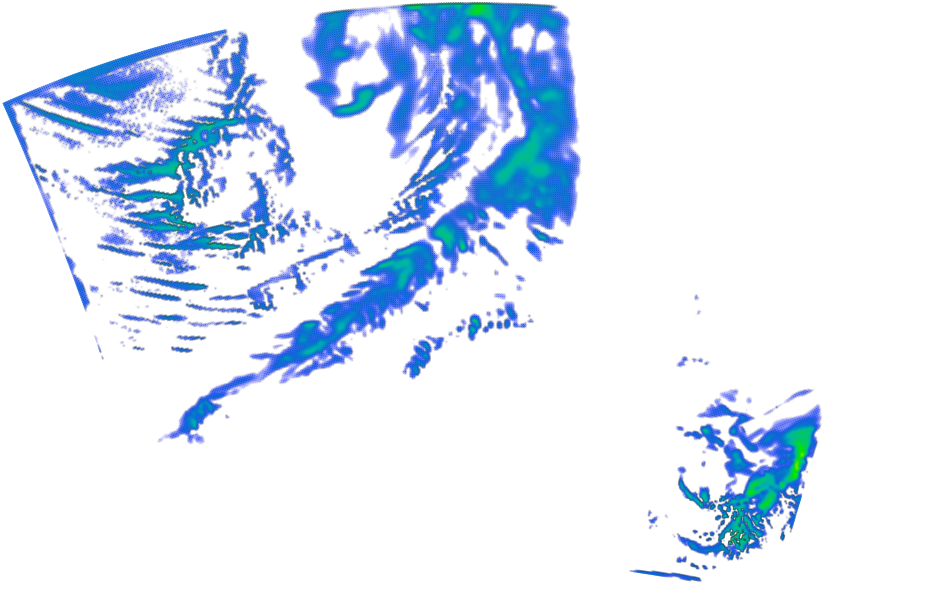
\includegraphics[scale=0.4]{Data/Mdrd_ukazka.png}
		\caption{Bitmapy od Medard-online \cite{medard}}
	\end{figure}
	
	\begin{itemize}
		\item \url{http://www.medard-online.cz/apiforecast?run=210313\_06\&forecast=precip\&layer=eu\&step=13}
	\end{itemize}
	
	\subsection{Radar.bourky}
	
	Radar.bourky \cite{chmi} je datový zdroj který poskytuje data prostřednictvím snímků z radaru, data jsou tedy ve formátu bitmap a obsahují velice detailní předpověď. Tento datový zdroj je prakticky nepoužitelný pro určování budoucího počasí, protože poskytuje data pouze v aktuálním čase, mimo srážky neposkytuje jiné prvky počasí a také pokrývá pouze Českou republiku s blízkým okolím.
	
	Na druhou stranu tento zdroj uchovává informace o srážkách tři dny dozadu s časovým rozdílem pouhých 10 minut. Díky tomu se dá tento zdroj použít pro přesné zobrazení srážek v minulosti případně odhad počasí v následujících hodinách na základě velice přesného posunu hodnot na snímcích.
	
	Proto se zdroj využívá pouze pro určení srážek v aktuálním čase případně následujících pár hodinách nebo pro určení srážek v minulých dnech s přesným posunem po deseti minutách.
	
	Ukázka odkazu který vrací bitmapu obsahující data o počasí pro Česko v jednom aktuálním čase. Součástí ukázky je i samotná bitmapa \emph{Radar.bourky\_bitmapa} \cite{chmi}. Při využívání tohoto API je zapotřebí zadat čas požadovaného snímku tento čas je vždy ve formátu {\it YYYYMMDD.HHMM}. Nejnovější snímek z radaru je vždy ten z aktuálního času zaokrouhlený dolů na desítky minut.
	
	\begin{figure}[b!]
		\centering
		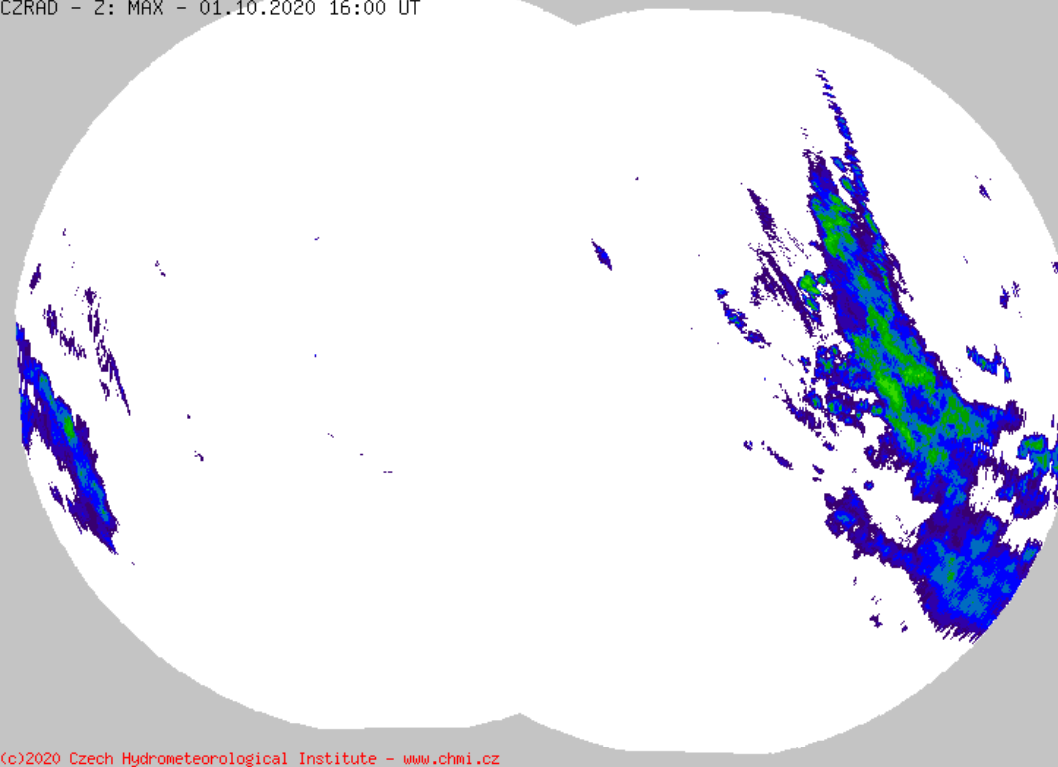
\includegraphics[scale=0.4]{Data/Rb_ukazka.png}
		\caption{Snímek z radaru od Radar.bourky \cite{chmi}}
	\end{figure}
	
	\begin{itemize}
		\item \url{http://radar.bourky.cz/data/pacz2gmaps.z\_max3d.20201001.1600.0.png}
	\end{itemize}
	
	\section{Shrnutí použitých zdrojů}
	
	Spousta datových zdrojů poskytujících data ve formě textu umožňuje poskytování dat jak v JSON tak XML formátu. Rovněž tak poskytují i informace o meteorologických prvcích jako rychlost a směr větru, čas východu a západu slunce nebo pocitovou teplotu vůči reálné teplotě. V práci se využívaly jen 4 základní prvky předpovědi a jen jeden předem zvolený způsob formátování dat. Proto se v tabulce shrnutí použitých zdrojů zobrazují pouze využívané prvky samotnou agregační knihovnou a jen jeden zvolený typ poskytnutých dat.
	
	\begin{table}[h]
		
		\captionof{table}{Shrnutí vlastností datových zdrojů}
		
		\begin{tabular} {l r c c c c c c c}
			
			Název & Typ dat & Počet dnů & Hodinový rozdíl & Stažení/min & Plocha & Prvek \\
			\hline
			Yr.no & XML & 9 & 1 a 6 & & svět & s,v,t1,t2 \\ 
			OpenWeatherMap & JSON & 5 & 3 & 60 & svět & s,v,t1,t2 \\ 
			WeatherUnlocked & JSON & 5 & 3 & 75 & svět & s,v,t1,t2 \\ 
			Medard-online & BMP & 5 & 1 &  & Evropa & s,t1 \\ 
			Radar.bourky & BMP & -3 & 0.16 (10 min)& & ČR & s \\ 
			
			\multicolumn{7}{r}{\footnotesize *s = srážky, v = vlhkost, t1 = teplota, t2 = tlak}\\
			
		\end{tabular}
	\end{table}
	
	\chapter{Agregace dat}
	
	Při agregaci dat bylo zapotřebí vyřešit pár otázek. První z nich byla potřeba jednotného výstupního formátu pro různorodá vstupní data, jako tento formát byly zvoleny bitmapy obsahující data o jednom prvku počasí, data jsou reprezentována pomocí barev a pokrývají určitou plochu pro určitý čas. Další otázkou bylo jak převádět barvy na číselné hodnoty a hodnoty zpět na barvy, tento problém vyřešilo využití škál. A nakonec byla potřeba pokrýt celou bitmapu daty pokud známe hodnotu počasí pro určité body, což nám vyřešila triangulace v kombinaci s interpolací.
	
	Každý z datových zdrojů je v agregaci dat realizován pomocí samostatné knihovny. Tato knihovna musí vždy implementovat rozhraní DataLoader a může využívat různé pomocné třídy pro správu dat o počasí jako je například triangulace nebo převod číselných hodnot na barvy a naopak. Dll soubor každé z knihoven je uložen do složky s datovými zdroji a následně je každá z knihoven datových zdrojů dynamicky načtena a zpracována pomocí reflexe třídou spravující agregaci dat.
	
	\section{Škála}
	
	Vzhledem k tomu že veškerá data o počasí jsou uložena do bitmap, ve který jsou data reprezentována barvou pixelů vzniká potřeba převádění barvy na číselnou hodnotu a naopak. Práce proto obsahuje metody, které pro určitou barvu vrátí desetinné číslo a pro určité číslo zase barvu.
	
	Nejprve tyto metody obsahovaly desítky podmínek které staticky kontrolovaly zda se jedná o konkrétní barvu, později zda barva patří do určitého rozmezí pro R, G, B složky. Tento přístup ale není vhodný, protože při potřebě změnit barvy pro určitá desetinná čísla vznikala nutnost přepsat hodnoty barev pro všechny metody ve veškerých podmínkách.
	
	Finálním řešením se stalo využití škál, škály jsou obrázky široké přesné tolik pixelů kolik hodnot uchovávají, kde každý pixel obsahuje unikátní barvu a reprezentuje jednu konkrétní číselnou hodnotu kterou daná barva reprezentuje. Výška škály může být pouze 1 pixel. Výhodou škál je, že změny barev reprezentujících hodnoty případně změny rozsahu uchovávaných hodnot se dá docílit pomocí použití nové škály která bude opět orientovaná na šířku. Další z výhod je, že metody které vrací hodnotu z barvy nemusí obsahovat desítky podmínek a stačí pouze vrátit hodnotu uloženou pro pixel. V programu jsou barvy ze škály uložený do slovníku, kde klíč reprezentuje barva a hodnotu desetinné číslo. Pro určení čísla z barvy stačí vypočítat index na kterém barva leží a tuto barvu vrátit.
	
	\section{Triangulace}
	
	Při vytváření bitmap dochází k určování hodnot počasí (teplota, srážky atp.) pro konkrétní zeměpisné souřadnice, které jsou následně převedeny na pixely bitmapy. Zjišťovat hodnotu pro každý jednotlivý pixel by bylo časově velice náročné, a protože můžeme předpokládat že v okolí pixelu budou obdobné hodnoty jako na pixelu samotném. Stačí nám tedy určit hodnoty pouze pro určité množství pixelů rozložených správně po bitmapě. Následně je potřeba tyto pixely nějakým způsobem propojit a dopočítat obsah mezi nimi, zde nám problém řeší využité triangulace.
	
	V práci se využívá S-hull Algoritmus pro triangulaci. Konkrétně Phil Atkinova implementace pro C\# \emph{S-hull} \cite{shull}. Algoritmus nám množinu bodů, v našem případě pixelů, rozdělí na trojúhelníky. Respektive nám pro každý vrchol řekne s kterými vrcholy je spojen hranou, čímž nám vznikne síť trojúhelníků pokrývající většinu bitmapy.
	
	%\vfill
	
	S-hull algoritmus slouží pro vytvoření Delaunayovi triangulace z množiny 2D bodů s časovou složitostí $O(n  log(n))$. Algoritmus využívá radiálního šíření, které se postupně vytváří z radiálně seřazené množiny 2D bodů, a je zakončen převracením trojúhelníků čímž se získá Delaunayova triangulace. Tento algoritmus ve srovnání s Q-hull algoritmem dosahuje přibližně polovičního času při vytváření triangulace pro náhodně generované množiny 2D bodů. S-hull je pro množinu unikátních 2D bodů $x_i$ implementován následovně:
	\begin{enumerate}
		\item Vybere počáteční bod $x_0$ z množiny bodů $x_i$.
		\item Seřadí body dle vzdálenosti od tohoto bodu $|x_i - x_0|^2$.
		\item Nalezne bod $x_j$, který je k bodu $x_0$ nejblíž.
		\item Nalezne bod $x_k$, který vytvoří nejmenší kružnici opsanou s body $x_0$ a $x_j$, současně i zaznamená střed kružnice opsané $C$.
		\item Seřadí body $x_0$, $x_j$, $x_k$ a za pomocí pravidla pravé ruky \cite{rhs} je získán počáteční prvek pro convex hull.
		\item Přetřídí zbývající body na základě vzdálenosti bodů od středu kružnice opsané $|x_i - C|^2$ pro získání bodů $s_i$.
		\item Postupně se přidávají body $s_i$ do rostoucího 2D convex hull který je závislý na trojúhelníku vytvořeném z bodů $x_0$, $x_j$, $x_k$. Následně jsou přidány zkosené hrany pro 2D-hull, které jsou bodu viditelné z nově vytvořených trojúhelníků.
		\item Vzájemně se nepřekrývající triangulace pro množinu bodů je nyní vytvořena. Tato metoda je velice rychlá mezi způsoby vytváření 2D triangulace.
		\item Sousední páry trojúhelníků této triangulace musí být \uv{převráceny} aby došlo k vytvoření Delaunayovi triangulace z počáteční nepřekrývající se triangulace.
	\end{enumerate}
	
	\begin{figure}[h]
		\centering
		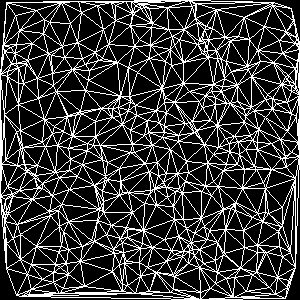
\includegraphics{Data/bmp_triangulace.png}
		\caption{S-hull pro 500 náhodně generovaných bodů v matici 300x300}
	\end{figure}
	
	\section{Interpolace}
	
	Bitmapa je pokryta sítí trojúhelníků kde známe hodnotu $Value$ každého vrcholu $V$. Nyní vzniká potřeba každý trojúhelník vyplnit barvami, které reprezentují hodnotu pixelů uvnitř trojúhelníku. Tuto práci řeší využití interpolace, neboli výpočet hodnoty uvnitř objektu na základě vzdálenosti od vrcholů.
	
	Pro výpočet interpolace postačí jednoduchý vzorec \emph{Interpolace v trojúhelníku} \cite{interp}, který na základě hodnot vrcholů trojúhelníku a vzdálenosti od nich pro zjišťovaný bod určí jakou hodnotu sám zjišťovaný bod má.
	
	%\vspace{10mm}
	
	V prvním kroku výpočtu je zapotřebí spočítat vzdálenost $Distance$ zjišťovaného bodu $P$ od všech tří vrcholů trojúhelníku $V_1$, $V_2$, $V_3$ (\ref{eq_dist}). 
	\newpage
	\begin{displaymath}
		Distance_{v1} =\sqrt{(V_{1x}-P_x)^2+(V_{1y}-P_y)^2}
	\end{displaymath}
	\begin{displaymath}
		Distance_{v2} =\sqrt{(V_{2x}-P_x)^2+(V_{2y}-P_y)^2}
	\end{displaymath}
	\begin{equation}\label{eq_dist}
		Distance_{v3} =\sqrt{(V_{3x}-P_x)^2+(V_{3y}-P_y)^2}
	\end{equation}
	
	Následně se určí váha každého vrcholu $W$, neboli inverzní hodnota jeho vzdálenosti od zjišťovaného bodu (\ref{eq_w1}).
	
	\begin{equation}\label{eq_w1}
		W_{v1} =\frac{1}{Distance_{v1}}
		\quad\mathrm{ }\quad 
		W_{v2} =\frac{1}{Distance_{v2}}
		\quad\mathrm{ }\quad 
		W_{v3} =\frac{1}{Distance_{v3}} 
	\end{equation}
	
	Ve finální části výpočtu se určí hodnota našeho zjišťovaného bodu $Value_p$, která je úměrná podílu součtu součinů vah a hodnot jednotlivých vrcholů trojúhelníku se součtem jednotlivých vah (\ref{eq_val}).
	
	\begin{equation}\label{eq_val}
		Value_v = \frac{W_{v1}Value_{v1} + W_{v2}Value_{v2} + W_{v3}Value_{v3}}{W_{v1} + W_{v2} + W_{v3}}
	\end{equation}
	
	\section{Složky zdrojů}
	
	Každý z datových zdrojů má svou vlastní složku ze které čte a do které si ukládá informace.
	
	V této složce se nachází konfigurační JSON soubor obsahující informace na základě kterých si služba nastaví své parametry při vytvoření instance. Mezi tyto informace patří název datového zdroje včetně zkratky. Zeměpisné souřadnice zpracovávané plochy. Maximální dovolený počet stažení dat za minutu. Počet hodin který má služba zpracovávat zpětně, minimální potřebný hodinový rozdíl pro nové stažení dat a především poslední čas zpracování dat. Na základě posledního času zpracování bitmap a minimálního potřebného hodinového rozdílu si datový zdroj při požadavku na vytvoření nových bitmap určí zda dojde k jejich vytváření či nikoli.
	
	Pokud zpracovává datový zdroj informace ve formě bitmap obsahuje tato složka i škálu daného datového zdroje. Pomocí této škály se převádí veškeré barvy na číselné hodnoty a následně za použití obecné škály služby se převádí čísla zpět na normalizovanou barvu.
	
	Nejdůležitější soubory ukládané do složek jsou samotné bitmapy s daty o počasí. Bitmapy si do své složky každý zdroj ukládá při požadavku na vytváření bitmap a následně je z této složky vrací při požadavku na poskytnutí dat o počasí pro daný prvek a čas.
	
	\section{Zpracovávání dat}
	
	Při zpracování dat do bitmap záleží na tom jakým způsobem jsou data datovým zdrojem poskytována.
	
	Pokud jsou data poskytována ve formě bitmap potřebujeme zjistit jakou škálou jsou data v bitmapě zobrazena a rozsah zpracované plochy. Následně se musí bitmapa přeškálovat, tedy jednotlivé pixely jsou převedeny na číselnou hodnotu pomocí škály zdroje a následně jsou čísla převedeny zpět na barvu za pomocí obecné škály pro agregaci dat využívané pro všechny zdroje na správu dat. Nakonec je potřeba správně pozicovat bitmapu. Na základě zeměpisných souřadnic rohů bitmapy se zjistí jaká plocha je zpracována. Pokud je plocha příliš velká tak jak tomu je u zdroje Medard, dochází k vyřezání požadované části a následnému roztažení na 728x528 pixelů. Naopak u zdroje Radar.bourky je plocha příliš malá a tak dochází k patřičnému zmenšení bitmapy ze zdroje a napozicování do finální větší bitmapy.
	
	Data poskytována ve formátu XML či JSON se zpracovávají jiným způsobem. Nejprve měla každá služba svůj seznam měst nacházejících se ve zpracovávané ploše pro který poskytuje informace o počasí. Pro každé z těchto měst se určilo počasí a pozice pixelu reprezentujícího dané město. Pixel se následně vykreslil na mapu a pomocí triangulace se vytvořila síť trojúhelníků, které se ve finále vybarvily. Tento způsob nebyl vhodný protože nepokrýval celou bitmapu rovnoměrně, v určitých místech chyběly informace a naopak v jiným místech bylo příliš mnoho bodů u sebe, proto se způsob zpracování změnil.
	
	Aktuálně dochází k cyklickému průchodu bitmapou s posunem 25 pixelů na výšku a šířku (\ref{bmpBody}). Každý z těchto pixelů je převeden na zeměpisné souřadnice na základě vzdálenosti od levého horního rohu přičemž dochází k určení počasí v tomto bodě. Počasí je následně uloženo do slovníku kde klíč tvoří čas dané předpovědi a hodnotou je list počasí pro stejný čas v různých bodech. Nakonec je pro každý z časů proveden průchod listem předpovědí a následuje vytvoření sítě trojúhelníků (\ref{bmpTriang}) pomocí triangulace zakončená vybarvením jednotlivých trojúhelníků využitím interpolace (\ref{bmpColors}) a vykreslení těchto barev do bitmapy. Pro každý čas je vytvořeno tolik bitmap kolik prvků počasí daná služba zpracovává. Počet jednotlivých časů je úměrný počtu všech dostupných předpovědí pro jednotlivé body.
	
	Použití triangulace není při zpracovávání rovnoměrně vzdálených bodů nutné, každopádně se v práci pro zpracování dat ponechala. Datové zdroje takto mohou zpracovávat i nerovnoměrně vzdálené body a pokud by došlo ke změně implementace určení dat v daných bodech, tedy pro jednotlivé časy by se body neurčovali cyklicky ale opět pomocí seznamu různě umístěných měst ve zpracované ploše, triangulace by se postarala o rozdělení bodů na síť trojúhelníků s následným vybarvením pomocí interpolace.
	
	\begin{figure}
		\centering
		
\includegraphics[scale=0.5]{Data/bmp_body.png}
		\caption{Body reprezentující teplotu na ploše}
		\label{bmpBody}
	\end{figure}
	
	\begin{figure}
		\centering
		
\includegraphics[scale=0.5]{Data/bmp_sit.png}
		\caption{Síť trojúhelníků pro bitmapu teploty}
		\label{bmpTriang}
	\end{figure}
	
	\begin{figure}
		\centering
		
\includegraphics[scale=0.5]{Data/bmp_vybarvena.png}
		\caption{Kompletní bitmapa pro teplotu}
		\label{bmpColors}
	\end{figure}
	
	\section{Ukládání dat}
	
	Veškerá zpracovaná data je potřeba uložit aby bylo možné je posléze poskytovat a nemuseli se pravidelně při každém dotazu o data generovat znovu. Vzhledem k tomu že se ukládají data o počasí na ploše nemá smysl používat žádnou databázi protože by bylo zbytečně složité ukládat celou předpověď pro každý bod zvlášť i když by bod vedle obsahovat obdobné, ne-li úplně totožné údaje. Právě proto se zvolilo ukládání dat do bitmap které nám jednoduše pokryjí celou zpracovanou plochu.
	
	Výhodou bitmap je, že pro jeden zvolený čas mohou pokrýt velkou plochu a tím pádem stačí jeden soubor pro určitý čas. Nevýhodou je, že bitmapa nám poskytuje data pouze o jednom prvku počasí, například o teplotě, a proto pokud chceme zjišťovat více vlastností počasí v jedno chvíli musíme pro každý prvek uložit jednu samostatnou bitmapu s těmito daty.
	
	Jednotlivé datové zdroje ukládají své bitmapy se jménem {\it TYP-ČAS} a na základě tohoto jména je následně možné bitmapy vracet. Prefix názvu matice pojmenovaný jako {\it TYP} reprezentuje prvek předpovědi která bitmapa zpracovává, pro teplotu to je $TEMP$, srážky $PREC$ a tak podobně. V druhé části názvu zvané $ČAS$ je uložený čas předpovědi, pro většinu datových zdrojů ve formátu {\it ROK-MĚSÍC-DEN-HODINA}. Vzhledem k tomu že datové zdroje poskytují předpovědi pro časy vzdálené v řádu hodin je zbytečné ukládat do názvu času minuty nebo sekundy. Pouze jediný z datových zdrojů Radar.bourky poskytuje data o počasí v rámci minut s posunem po 10 minutách a proto je pro tento zdroj zahrnut i parametr minut v časové části názvu {\it ROK-MĚSÍC-DEN-HODINA-MINUTA}.
	
	To pro jakou plochu datové zdroje zpracovávají své bitmapy je dopředu určeno a proto nemá smysl tento údaj ukládat přímo do bitmap.
	
	Každý z datových zdrojů ukládá do své složky zpracované bitmapy a následně při určitých dotazech tyto bitmapy vrací. 
	
	\section{Poskytování dat}
	
	Datové zdroje po obdržení informací o prvku počasí a času dokáží vrátit správnou bitmapu, která je vybrána dle svého názvu. Název prvku počasí se musí shodovat s prefixem názvu bitmapy {\it TYP}. Požadovaný čas předpovědi si každý z datových zdrojů umí správně zaokrouhlit aby bylo jasné jaká bitmapa tento čas zpracovává. Pokud datový zdroj poskytuje data každých 10 minut je čas zaokrouhlen na desítky minut dolů. Při poskytování dat každou hodinu je k času přičteno 30 minut a následně je tento čas zaokrouhlen na hodiny dolů. Poslední možností je vracení času jednou za 3 nebo 6 hodin, v tomto případě se zjistí ke které časové hranici má zadaný čas blíže a tato varianta je zvolena.
	
	Zaokrouhlený čas je následně převeden do formátu {\it ROK-MĚSÍC-DEN-HODINA}, případně včetně $MINUTA$ pro Radar.bourky. V tuto chvíli zná datový zdroj celý název hledané bitmapy a tu jednoduše vrátí. Pokud bitmapa neexistuje dojde k vyvolání výjimky.
	
	Pokud datový zdroj vytváří bitmapy nekonzistentně, například prvních pár dnů je s rozestupem 1 hodiny a zbytek s rozestupem 6 hodin tak jak to dělá například Yr.no, dochází při nenalezení bitmapy se zaokrouhleným časem k sekvenčnímu průchodu všech zpracovaných bitmap a vrácení bitmapy s nejbližším časem k požadovanému času. Tato bitmapa je vrácena pouze tehdy pokud je odchylka času maximálně 6 hodin v opačném případě dochází opět k vyvolání výjimky.
	
	\chapter{Distribuce dat}
	
	Shromážděné a zprůměrované předpovědi počasí je potřeba nějakým způsobem dodávat klientovi. Tuto úlohu nám splní webová služba, která pro různé dotazy ve formě url API vrací agregovaná data o počasí v požadovaných formátech. Služba se implementovala jako MVC aplikace pro C\# a využívá pro svou práci knihovnu pro agregaci dat z předešlé sekce. Vzhledem k tomu, že jsou data o počasí uložená do bitmap, lze informace o počasí poskytovat i bez připojení k internetu, musíme však mít pro dané časy bitmapy dopředu vytvořené. Služba volá požadavek na vytvoření nových bitmap vždy při spuštění a následně každou další hodinu běhu, jednotlivé datové zdroje si následně zjistí kdy byly bitmapy naposledy vytvořený a pokud již uplynul minimální čas dojde k vytváření bitmap nových, tento čas se může u každého datového zdroje lišit.
	
	\section{API}
	
	Při práci se službou je využíváno webové API které pro správně zadané vstupní parametry vrací požadovaná data. Webová služba poskytuje data o počasí ve třech formátech XML, JSON a BMP. Dále lze získat souřadnice ohraničující maximální plochu předpovědi a nakonec je možné získat jednotlivé škály, které služba využívá pro správu dat o počasí v bitmapách.
	
	\section{Bitmap předpověď}
	
	Tato předpověď se získává požadavkem $bmp$ a vždy vrací bitmapu o rozměrech 728x528 pixelů pokrývající určitou plochu. Plocha je vymezená body zeměpisných souřadnic, konkrétně levým horním $p1$ a pravým dolním $p2$ rohem. Pokud nedojde k zadání těchto bodů je bitmapa určena pro maximální možnou plochu. Při určování této předpovědi je rovněž zapotřebí i čas pro který se má předpověď určit $time$, tento čas musí být ve formátu ISO 8601 a pokud není zadán nebo je místo něj vyplněna hodnota 0 určí se předpověď pro aktuální čas. Následně je potřeba zadat prvek předpovědi $type$, který má bitmapa reprezentovat. Tyto prvky jsou 4, prvek $prec$ reprezentuje srážky [mm], prvek $temp$ teplotu [°C], $pres$ tlak [hPa] a $humi$ vlhkost [\%]. Nakonec se zadávají datové zdroje $loaders$, takzvané loadery, ze kterých má služba získávat data. Je potřeba zadat zkratky loaderů oddělené čárkami pro každý loader který má služba využít pokud není zadán žádný loader použijí se všechny dostupné datové zdroje současně.
	\\\\
	\url{adresaserveru/bmp?type={typ}\&time={čas}\&loaders={datové\_zdroje}\&p1={bod1}\&p2={bod2}}
	
	\begin{center}
		
		\captionof{table}{Parametry bitmap předpovědí}
		
		\begin{tabular}{c c p{13cm}}
			Název & Povinnost & Význam \\
			\midrule
			type & ANO & Typ předpovědi, určuje prvek vykreslených informací. Například prvek $prec$ reprezentuje srážky v milimetrech a prvek $temp$ teplotu ve stupních Celsia.\\ 
			time & NE & Čas předpovědi, pokud je zadán musí být ve formátu ISO 8601. Pokud zadán není nebo je zadána hodnota 0  určí se předpověď pro aktuální čas.\\ 
			loaders & NE & Datové zdroje které se mají použít. Výběr datových zdrojů se provede zadáním zkratek jednotlivých zdrojů oddělených čárkami. Pokud je parametr prázdný použijí se veškeré datové zdroje služby. \\ 
			p1 & NE & Levý horní roh vymezující plochu bitmapy. Bod reprezentuje zeměpisné údaje v pořadí zeměpisná šířka a délka (latitude a longitude), údaje jsou odděleny čárkou. Pro oddělení celé a desetinné části souřadnice se používá tečka. Pokud bod $p1$ není zadán, bitmapa se vykreslí pro celou možnou plochu.\\
			p2 & NE & Pravý dolní roh vymezující plochu bitmapy. Bod reprezentuje zeměpisné údaje v pořadí zeměpisná šířka a délka (latitude a longitude), údaje jsou odděleny čárkou. Pro oddělení celé a desetinné části souřadnice se používá tečka. Pokud bod $p2$ není zadán, bitmapa se vykreslí pro celou možnou plochu.\\
		\end{tabular}
	\end{center}
	
	Příklady požadavků:
	\begin{itemize}
		\item Požadujeme bitmapu s daty o teplotě pro aktuální čas, která pokrývá celou možnou plochu a využívá veškeré datové zdroje.
		
		\url{adresaserveru/bmp?type=temp}
		
		\item Požadujeme bitmapu s daty o srážkách pro 26. 5. 2021 18:30, která pokrývá celou možnou plochu a využívá datové zdroje od služeb OpenWeatherMap a Yr.No.
		
		\url{adresaserveru/bmp?type=prec\&time=2021-05-26T18:30:00\&loaders=owm,yrno}
		
		\item Požadujeme bitmapu s daty o srážkách pro aktuální čas, která pokrývá město Olomouc a využívá datový zdroj od služby Medard-Online.
		
		\url{adresaserveru/bmp?type=prec\&p1=49.621559,17.1507294\&p2=49.5211889,17.4213141\&loaders=mdrd}
	\end{itemize}
	
	\section{XML a JSON předpověď}
	
	Tento požadavek nám dovoluje získat data o počasí pro určitý bod v zadaném čase, případně lze určit data o počasí pro více časů za sebou s konstantním hodinovým rozdílem. Při získávání XML nebo JSON dat potřebujeme zadat stejně jako u bitmap předpovědí zadat parametr požadovaného času $time$ a datové zdroje které tento čas zpracovávají $loaders$. Dále musíme zadat požadovaný formát dat XML/JSON $data$ a zeměpisný bod pro který chceme počasí určit, bod se skládá z parametrů $lon$ a $lat$. Pro získání více časových oken v jedné předpovědi musíme přidat parametr reprezentující počet předpovědí $numOfFcs$ a hodinový rozdíl mezi těmito předpověďmi $hourDif$.
	\\\\
	\url{adresaserveru/{data}?time={čas}\&lat={zeměpisná\_šířka}\&lon={zeměpisní\_délka}\&loaders={datové\_zdroje}}
	
	\begin{flushleft}
		\url{adresaserveru/{data}?time={čas}\&numOfFcs={počet\_předpovědí}\&hourDif={hodinový\_rozdíl\_mezi\_předpověďmi}\&lat={zeměpisná\_šířka}\&lon={zeměpisní\_délka}\&loaders={datové\_zdroje}}
	\end{flushleft}
	
	\begin{center}
		
		\captionof{table}{Parametry XML/JSON předpovědí}
		
		\begin{tabular}{c c p{13cm}}
			Název & Povinnost & Význam \\
			\midrule
			data & ANO & Formát v jakém mají být data o počasí zpracována. Rozlišujeme dva typy a to $xml$ a $json$.\\
			lon & ANO & Longitude, parametr reprezentující zeměpisnou délku požadované souřadnice. Desetinná a celá část souřadnice jsou odděleny tečkou.\\
			lat & ANO & Latitude, parametr reprezentující zeměpisnou šířku požadované souřadnice. Desetinná a celá část souřadnice jsou odděleny tečkou.\\
			time & NE & Čas předpovědi, pokud je zadán musí být ve formátu ISO 8601. Pokud zadán není nebo je zadána hodnota 0  určí se předpověď pro aktuální čas.\\ 
			loaders & NE & Datové zdroje které se mají použít. Výběr datových zdrojů se provede zadáním zkratek jednotlivých zdrojů oddělených čárkami. Pokud je parametr prázdný použijí se veškeré datové zdroje služby. \\
			numOfFcs & NE & Počet časových oken které má předpověď obsahovat. Pokud není tento parametr zadán, v předpovědi bude právě jedno časové okno pro zadaný čas.\\
			hourDif & NE & Hodinový rozdíl mezi jednotlivými časovými okny v předpovědi. Pokud není tento parametr zadán, v předpovědi bude právě jedno časové okno pro zadaný čas.\\
		\end{tabular}
	\end{center}
	\newpage
	Příklady požadavků:
	\begin{itemize}
		\item Požadujeme předpověď o počasí pro aktuální čas v Ostravě zpracovanou všemi datovými zdroji ve formátu XML.
		
		\url{adresaserveru/xml?lon=18.262524\&lat=49.820923}
		
		\item Požadujeme předpověď o počasí pro datum a čas 14.03.2021 18:35 v Ostravě zpracovanou všemi datovými zdroji ve formátu JSON.
		
		\url{adresaserveru/json?lon=18.262524\&lat=49.820923\&time=2021-03-14T18:35:00}
		
		\item Požadujeme předpověď o počasí pro datum a čas 14.03.2021 18:35 v Ostravě zpracovanou datovými zdroji OpenWeatherMap a WeatherUnlocked ve formátu XML.
		
		\url{adresaserveru/xml?lon=18.262524\&lat=49.820923\&time=2021-03-14T18:35:00\&loaders=owm,weun}
		
		\item Požadujeme předpověď o počasí v Ostravě pro 5 časových oken s 3 hodinovými rozestupy počínaje aktuálním časem ve formátu JSON.
		
		\url{adresaserveru/json?lon=18.262524\&lat=49.820923\&time=2021-03-14T18:35:00\&numOfFcs=5\&hourDif=3}
		
	\end{itemize}
	
	\section{Ohraničení bitmapy}
	
	Služba vytváří bitmapy pro určitou plochu. Aby bylo možné zjistit jaké maximální ohraničení bitmapy můžeme zadávat, respektive jakou plochu bitmapa pokrývá pokud žádné parametry hranic nezadáme, máme možnost získat JSON data obsahující maximální ohraničení bitmapy tedy levý horní roh $TopLeftCornerLonLat$ a pravý dolní roh $BotRightCornerLonLat$. Oba body obsahují konkrétní hodnoty zeměpisné délky $Lon$ a šířky $Lat$.
	
	Příklad požadavku:
	\begin{itemize}
		\item Požadujeme škálu pro teploty.
	
		\url{adresaserveru/bounds}
	\end{itemize}

	\section{Využívané škály}
	
	Při stahování bitmap obsahujících data o počasí je vhodné mít prostředek na převod barev z jednotlivých pixelů na číselné hodnoty. Právě pro tento účel slouží škály.
	
	Služba nám proto umožňuje stažení jednotlivých škál, které používá při zpracovávání bitmap s daty o počasí. Stačí znát zkratku prvku počasí a služba nám vrátí využívanou škálu.
	\newpage
	Příklady požadavků:
	\begin{itemize}
		\item Požadujeme škálu pro teploty.
		
		\url{adresaserveru/scale?type=temp}
		
		\item Požadujeme škálu pro srážky.
		
		\url{adresaserveru/scale?type=prec}
		
	\end{itemize}
	
	\section{Zkratky prvků počasí}
	
	Zkratky pro jednotlivé prvky předpovědí které se využívají v parametru $type$.
	
	\begin{center}
		
		\captionof{table}{Zkratky prvků předpovědí}
		
		\begin{tabular}{c c c}
			Prvek počasí & Jednotka & Zkratka pro API\\
			\midrule
			Srážky & mm & prec \\
			Teplota & °C & temp \\
			Tlak & hPa & pres \\
			Vlhkost & \% & humi \\
		\end{tabular}
	\end{center}
	
	\section{Zkratky datových zdrojů}
	
	Zkratky pro jednotlivé datové zdroje které se využívají v parametru loaders. Při použití více zkratek za sebou oddělených čárkou dojde k použití více zdrojů současně.
	
	\begin{center}
		
		\captionof{table}{Zkratky datových zdrojů}
		
		\begin{tabular}{c c}
			Celý název datového zdroje & Zkratka pro API\\
			\midrule
			Radar.bourky & rb \\
			Medard-online & mdrd \\
			OpenWeatherMap & owm \\
			Yr.no & yrno \\
			WeatherUnlocked & weun \\
		\end{tabular}
	\end{center}
	
	\section{Chyba při zpracování dat}
	
	Při požadavku na dodání dat může dojít k chybě, nejčastěji při chybném zadání parametrů v API, případně i při požadování dat pro čas který ještě bitmapami není zpracován. Pokud tato situace nastane služba místo požadovaných dat vrátí text ve formátu JSON obsahující jediný atribut $message$ s informace proč k pádu došlo a jak parametry upravit aby se chyba neopakovala a bylo možné nějaké informace o počasí získat.
	
	\chapter{Vizualizace dat}
	
	Část vizualizace dat je realizována prostřednictvím desktopové aplikace Bude-hezky napsané v C\# Windows Forms. Aplikace umožňuje uživateli zobrazit informace o různých prvcích počasí v bodě či na trase pro zvolený čas. Předpověď je zároveň tvořena grafem a bitmapou barev pokrývající zobrazenou plochu. Data jsou distribuována webovou službou a uživatel si může zvolit které datové zdroje chce pro své předpovědi používat.
	
	\section{Obecné použití}
	
	Aplikace je tvořena několika vzájemně propojenými částmi a to mapou reprezentující plochu pro kterou chceme znát počasí, lištou času pro který nebo od kterého chceme počasí určit, radio buttony reprezentující prvek předpovědi, check boxy pro volbu datových zdrojů, grafem zobrazující počasí pro více časových intervalů, text boxem pro vybrání místa textem, tlačítkem pro přehrání animace počasí společně s nastavitelnými parametry této animace a nakonec meníčkem pro nastavení aplikace případně volby určitých akcí.
	
	Při používání aplikace si uživatel zvolí který prvek počasí chce zobrazit vybráním patřičného radio buttonu a které z datových zdrojů si přeje používat zakliknutím požadovaných check boxů. Následně je potřeba zvolit čas první předpovědi reprezentovaný spodní lištou. Při každé změně času, prvku počasí nebo datového zdroje dojde k vykreslení bitmapy na mapu. Bitmapa reprezentuje počasí na ploše a při změně zobrazené plochy nebo změně přiblížení se bitmapa patřičně překreslí.
	
	Prvky počasí odpovídají veškerým prvkům poskytovaným webovou službou, jedná se tedy o srážkám, teplotu, tlak a vlhkost. Pro datové zdroje se rovněž používají veškeré datové zdroje které služba poskytuje. Lišta dat a časů 
	je pokryta časy od šesti hodin zpět po 5 dnů dopředu od aktuálního času a krokuje se po deseti minutách.
	
	Při určování číselných hodnot z bitmap se využívají totožné škály které webová služba používá při vyvážení samotných bitmap. Tyto škály si vizualizační aplikace dokáže stáhnout a přepsat vybráním akce aktualizace v menu pokud dojde k jejich změně na straně webové služby.
	
	\section{Mapa}
	
	Pro vykreslení a práci s mapou se nejprve používala komponenta MapWinGIS která poskytovala veškeré potřebné vlastnosti, naneštěstí bylo zapotřebí tuto komponentu nejdříve na zařízení nainstalovat a až poté ji mohla aplikace využívat. Tento důvod způsobil nutnost výměny komponenty za konkurence schopnou alternativu.
	
	Pro práci s mapou se nakonec využívá komponenta GMap.NET, která je volně dostupná pro rozšíření vlastností Windows Forms prostřednictvím NuGet balíčků. Tato komponenta nám umožňuje vykreslit mapu po které se může uživatel pohybovat, přibližovat a oddalovat ji. Komponenta dokáže určit zeměpisné souřadnice bodu ve kterém se nachází kurzor myši, takže není problém určit souřadnice požadovaného místa a ani plochy pro kterou data určujeme protože ta je vyhrazena levým horním a pravým dolním rohem mapy. Komponenta nám dovoluje přidat značky s popisky na mapu pokud máme za potřebí vyznačit zjišťovaný bod či body na trase, pro trasu se krom bodů vykreslí i křivka reprezentující celou cestu. Do mapy máme také možnost vykreslit bitmapu což se využívá při zobrazení dat v celé ploše.
	
	Na samotné mapě se vždy při změnách času, prvku a zdrojů vykresluje bitmapa reprezentující počasí, průhlednost této bitmapy lze nastavit prostřednictvím volby v menu.
	
	\section{Počasí v bodě}
	
	Při určování počasí v bodě stačí dvakrát kliknout do mapy na místo kde chceme zjistit přesnou hodnotu počasí. Následně se na tomto bodě vykreslí značka s popiskem reprezentujícím hodnotu počasí v tomto bodě. Při opětovném kliknutí na značku dojde k jejímu odstranění. Součástí předpovědi je i zobrazení grafu pod mapou, graf reprezentuje počasí v zvoleném bodě od počátečního času, tedy času nastaveném na liště a každý další sloupec grafu zobrazuje počasí pro stejný bod v čase inkrementovaném o hodinu. Počet sloupců je nastavitelný. Součástí této předpovědi je i zobrazení tabulky s detailem o počasí popisujícím hodnoty různých prvků na následujících 5 dní, tento detail je možné v nastavení vypnout.
	
	Mimo znázorňování počasí dvojitým kliknutím lze bod vybrat i napsáním názvu hledaného místa do textového pole v pravé dolní části mapy. Pokud uživatel napíše do tohoto pole název místa a akci potvrdí enterem, dojde k vyhodnocení textu a převodu na pravděpodobně smýšlené body službou Mapbox \cite{mapbox} z kterých je vybrán ten nejvěrohodnější. 
	
	Při zjišťování počasí v bodě se využívají data z bitmapy kterou si aplikace stáhla z webového serveru ve chvíli co byl zvolen prvek počasí, datový zdroj a čas. Z této bitmapy se určí pixel obsahující data o počasí pro požadovaný bod a pomocí škály je RGB hodnota převedena na desetinné číslo.
	
	\section{Počasí na trase}
	
	Mimo počasí pro jeden bod v různých časem máme možnost vykreslit i počasí na určité trase, tedy na více různých bodech v rozdílných časech na základě rychlosti pohybu. Trasa se zadává pomocí předem vytvořeného GPX souboru obsahujícího body reprezentující samotnou trasu. Při zobrazování trasy je potřeba zjistit jakou rychlostí se po trase postupuje pro možnost zjištění postupu času na následující bodech zvolené cesty. Tato rychlost se v aplikaci může určit dvěma způsoby. Prvním je zadání počátečního času a dopravního prostředku, každý dopravní prostředek má svou vlastní předem nastavenou rychlost a při výpočtu uplynulé vzdálenosti od počátku dokážeme určit i čas v tomto uplynulém bodě. Druhým způsobem určení času na trase je zadání času začátku a konce cesty, díky těmto informacím dokážeme určit jak dlouho trvá urazit celou cestu a tím pádem dokážeme spočítat i rychlost, když známe délku cesty. Délka cesty se jednoduše spočítá jako součet vzdáleností v metrech mezi jednotlivými body trasy.
	
	Při požadavku o zobrazení počasí v trase musí uživatel vybrat možnost $Akce$ z menu a v něm zakliknout {\it Nahrát trasu z GPX souboru}. Poté si uživatel vybere jednu z možností určení rychlosti dopravy, zadá tedy počáteční čas a dopravní prostředek případně počáteční a koncový čas. Nakonec vybere cestu k samotnému GPX souboru ve svém počítači. Pokud během toho procesu dojde k jakékoliv chybě proces se ukončí a uživateli se vypíše co přesně neproběhlo během zobrazování trasy správně.
	
	Po úspěšném zadání všech parametrů a zpracování souboru je na mapě nakreslena křivka reprezentující trasu. Na křivce jsou vyznačeny značky začátku a cíle trasy, každá ze značek obsahuje detailní popis informací o trase. Barva křivky je určena hodnotou počasí v bodě na křivce. Každý ze zobrazených bodů zná svou hodnotu počasí, čas v bodě, vzdálenost od začátku a čas potřebný k průchodu trasou od začátku k tomuto bodu. Při najetí myší na trasu dochází k zobrazení výpisu těchto informací pro snadnější zjištění počasí na trase. Zároveň se při vykreslení trasy zobrazí v horní části mapy dvě nová tlačítka pro možnost nastavení nového času trasy případně odstranění trasy. Při změně datového zdroje nebo prvku počasí během toho co je trasa vykreslená dochází k zpracování nově zadaných hodnot a zobrazení nových dat na stejné trase včetně jejího přebarvení.
	
	Součástí zobrazení trasy je i vykreslení grafu pod mapou, graf obsahuje 10 sloupců kde každý sloupec reprezentuje jeden ze stejně vzdálených bodů na trase. Graf slouží jako rychlý náhled k určení postupu počasí na celé trase, zda má stoupající či klesající tendenci případně se příliš nemění.
	
	Určování dat o počasí v bodech trasy se provádí stejně jako v určování informací o počasí v bodě. Pro každý vykreslený bod na trase se použije stažená bitmapa na které se najde pixel reprezentující danou zeměpisnou souřadnici a pro tento pixel se určí hodnota počasí převodem RGB hodnoty na desetinné číslo prostřednictvím škály. Ke stahování nových bitmap dochází během zpracovávání trasy a to vždy při překročení času který poslední stažená bitmapa poskytuje.
	
	\section{Animace počasí}
	
	Uživatel má možnost zobrazit si animaci předpovědí pro zvolený prvek počasí od zvoleného počátečního času. Při kliknutí na tlačítko pro přehrání animace dochází k vykreslení bitmap předpovědí pro zvolený prvek počasí, čas počasí pro animaci začíná od zvoleného času na liště, následně se v animaci vykreslují nové bitmapy pro následující čas inkrementovaný o zvolený interval. Intervaly se pohybují v hodnotách 10min, 30min, 1h, 3h a 6h. Počet kroků animace je rovněž nastavitelný a dodává nám možnost zobrazit průběh počasí pro dlouhé či krátké úseky času. Při běhu animace můžeme vidět v jakém časovém úseku se právě nacházíme a kolikátý snímek z celkového počtu je aktuálně zpracováván.
	
	Při zpracování animace dochází k cyklickému stahování bitmap z webové služby. Hranice bitmapy jsou ohraničeny souřadnicemi rohů mapy a čas této předpovědi je vždy o zvolený časový interval vyšší než byl u předpovědi předešlá. Prvek počasí ani datové zdroje se u animace neliší ty jsou pro celou animaci stejné.
	
	\section{Graf}
	
	Součástí aplikace je i graf obsahující informace o předpovědích pro jednotlivé časy. Šířka grafu se dynamicky mění při změně rozměrů okna aplikace. Graf má na ose $y$ sloupce ukazující hodnotu daného prvku počasí v rozmezí od minima do maxima, na ose $x$ se nachází čas předpovědi pro daný sloupce. Graf je vykreslován na panel pomocí základních metod knihovny System.Drawing, pro tento účel se nevyužívají žádné externí knihovny. Barva sloupců společně s jejich počtem v grafu je nastavitelná.
	
	Při vykreslování grafu pro bod reprezentují všechny sloupce stejné místo s rozdílným časem. Časy jsou od sebe posunuté o hodinu a počet vykreslených sloupců lze změnit v nastavení.
	
	Pro tuto předpověď nám graf vykresluje počasí pro 8 rovnoměrně vzdálených míst na trase. Proto počet sloupců v tomto grafu je vždy 8. Na rozdíl od grafu pro předpověď v bodě nám tento graf na ose $x$ reprezentuje čas sloupce v aktuálním bodě a vzdálenost tohoto bodu od počátku cesty.
	
	Zobrazený typ jednotek předpovědi na ose $y$ se mění dle zvoleného prvku počasí v radio buttonech. Každý prvek předpovědi zná své jednotky a mimo to i minimální a maximální hodnotu počasí pro tuto jednotku. Hodnota předpovědi pro každý sloupec se tedy určí jako procentuální hodnota v rozmezí od minima po maximum.
	
	Pokud graf aktuálně nevykresluje žádné informace tak je v poli určeném pro sloupce vypsán text popisující co pole reprezentuje a kdy zde dojde k vykreslení dat. Nejprve bylo pole úplně prázdné a neobsahovalo žádný text čímž v aplikaci vznikla velká bílá plocha bez účelu, takto uživatel na první pohled ví k čemu zde tato plocha je. Tento text je v poli vypsán vždy při startu aplikace a následně při spuštění animace nebo při vymazání zobrazené předpovědi.
	
	\section{Nastavení a akce}
	
	Součástí aplikace je i menu nacházející se v horní liště. Menu je rozděleno do části $nastavení$ pro individuální změny aplikace a $akce$ pro rychlé volby.
	
	V části $nastavení$ lze nastavit adresu webové služby poskytující data o počasí. Dále se zde nachází možnost změny průhlednosti vykreslené bitmapy na samotnou mapu, lze vybrat vlastní hodnotu v rozmezí od 0 do 255 kde 0 je naprosto průhledná bitmapa a 255 bitmapa bez jakékoliv průhlednosti je zde i volba pro přímé nastavení minima či maxima bez potřeby zapisovat hodnotu ručně. Následně zde lze nastavit počet vykreslených sloupců v grafu při určování počasí v bodě. Všechny tyto hodnoty se musí nacházet v předem definovaném rozmezí od minima po maximum, při zadání neplatné hodnoty dojde k nastavení nejbližší platné. Nastavení obsahuje i možnost změny barvy sloupců grafu a nakonec zde lze i aktualizovat maximální hranice bitmapy nebo stáhnout nové škály z webové služby pro určování číselných hodnot z RGB pixelů. Při potřebě nastavení výchozích hodnot lze v nastavení zvolit i tuto variantu.
	
	Součástí tohoto nastavení byla i možnost změny počtu kroků při animaci a změna časového intervalu mezi jednotlivými kroky. Změny těchto parametrů se nakonec přesunuly přímo do aplikace vedle tlačítka pro spuštění animace. K této změně došlo protože se předpokládá že tyto parametry se budou pravidelně měnit a proto je zbytečné je mít schované v sekci s nastavením prvků které se změní pouze jednou případně velice výjimečně.
	
	V části menu $akce$ je na výběr mezi dvěma volbami. První je vykreslení cesty z GPX souboru pro zobrazení trasy s počasím. Druhou je možnost přemazání mapy při zobrazení nežádoucích dat. Tato volba slouží k vymazání všech hodnot v aplikaci. Při této volbě dojde k smazání grafu, bitmapy počasí na mapě a značce označující počasí v bodě, případně se odstraní trasa společně s jejími body a popisy.
	
	Veškeré nastavení aplikace se ukládá do konfiguračního JSON souboru. Při spuštění aplikace se z tohoto souboru načtou data o adrese serveru, průhlednosti bitmapy, ohraničení plochy, počtu kroků při animaci, počtu předpovědí pro počasí v bodě, poslední zvolený prvek počasí a naposledy zvolené datové zdroje. Díky tomuto souboru nemusí uživatel při každém spuštění znovu nastavovat veškeré věci znovu. Při změně jakéhokoliv z těchto atributů dochází k přepsání JSON souboru pro udržení neustále konzistence s aplikací po ukončení aplikace a opětovném spuštění.
	
	\section{Chyby při zobrazování dat}
	
	Pokud dojde k chybě při získávání dat ze serveru vypíše se chybová hláška vrácená samotnou službou jako atribut $message$ v chybovém JSON výstupu. K těmto chybám dochází nejčastěji při pokusu o získání počasí pro čas pro který nemá žádný ze zvolených datových zdrojů vytvořenou bitmapu. Případně při pokusu o zjištění počasí v bodě mimo zpracovávanou plochu. Pokud dochází k pádu z neznámého důvodu dochází k výpisu obecné chyby a prosba o kontrolu zda je webová služba aktuálně dostupná.
	
	Může se stát že dojde k chybě i při určování počasí trasy z GPX soboru. Mimo pád při neschopnosti zjištění počasí pro daný bod dochází i k chybě při zpracování samotného GPX soboru při nepodporovaném formátování. Případně dochází k chybě při zadání většího počátečního času než toho koncového. Při těchto chybách dochází k oznámení informace uživateli proč došlo k chybě a možnost napravení chyb při novém vykreslení trasy.
	
	\chapter{Závěr}
	
	Hlavní část této práce byla analýza různých datových zdrojů s daty o počasí a jejich následné využití pro poskytování vlastních agregovaných dat. Bylo zapotřebí zjistit jak každý ze zdrojů funguje a najít ideální řešení pro jeho využití v práci. Celá knihovna Agregace Dat byla vytvářena s předpokladem průběžného rozšíření o nové zdroje. Následně bylo zapotřebí najít ideální způsob poskytování zpracovaných dat pomocí webové služby, zjistit jak ideálně data ukládat a hledat. Nakonec se veškerá poskytovaná data zobrazila prostřednictvím vizualizační aplikace pro demonstraci možného využití dodávaných dat.
	
	Při zpracovávání této práce jsem se naučil jak psát více vzájemně kooperujících projektů současně. Pochopil jsem jakým způsobem služby s daty o počasí poskytují svá data a proč každá poskytuje své informace trochu jiným způsobem. Zjistil jsem jakým způsobem získávat data pomocí různých API a jak důležitý je jednoduchý a zároveň plně funkční návrh tohoto rozhraní. Ke konci práce jsem si uvědomil důležitost dobrého návrhu celé práce před samotnou realizací. Problémy vzniklé při změně funkcionality a složitém rozšíření některých částí se mohli s lepším návrhem řešit mnohem snadněji.
	
	\nocite{*}
	
	\printbibliography[title={Literatura}, heading=bibintoc]
	
	
\end{document}
